\subsection{Nombre del sistema de software}

El nombre del sistema de software que está siendo desarrollado por el Equipo A - Clifford como proyecto final de la materia Arquitectura de Software para el periodo académico 2019-01 es:
\begin{center}
    Kwii Platform
\end{center}

\subsection{Descripción del sistema de software}

Kwii Platform es un sistema de software que permite a sus usuarios comunicarse por medio de chats. Dichos chats crearán puntos de encuentro entre pares de usuarios o entre grupos de tres o más usuarios, donde pueden enviar mensajes de texto. Para acceder a los chats, se cuenta con dos interfaces amigables a los usuarios (uno para web y otro para teléfonos inteligentes), que están encargadas de permitir a los usuarios utilizar el sistema. El sistema notifica a los usuarios sobre la interacción de otros usuarios con ellos en estos chats, o sobre información importante que la plataforma quiera comunicarles.

\subsubsection{Descripción de idea del sistema de software para el curso de Arquitectura de Software}

Los usuarios interactúan con el sistema a través de los Kwiiers (interfaces gráficas de usuarios de la Kwii Platform), que les permite personificar a un Kwii. Un Kwii es un ser capaz de comunicarse con otros Kwiis (otros usuarios que personifican un Kwii), ya sea con un único Kwii o con un grupo de tres o más Kwiis. Los usuarios personifican a un único Kwii, y un único Kwii identifica de manera única a un usuario. Esta identificación única de los Kwiis es lograda a través de un sistema de autenticación y administración de usuarios, que contempla la Kwii Platform.
\begin{center}
    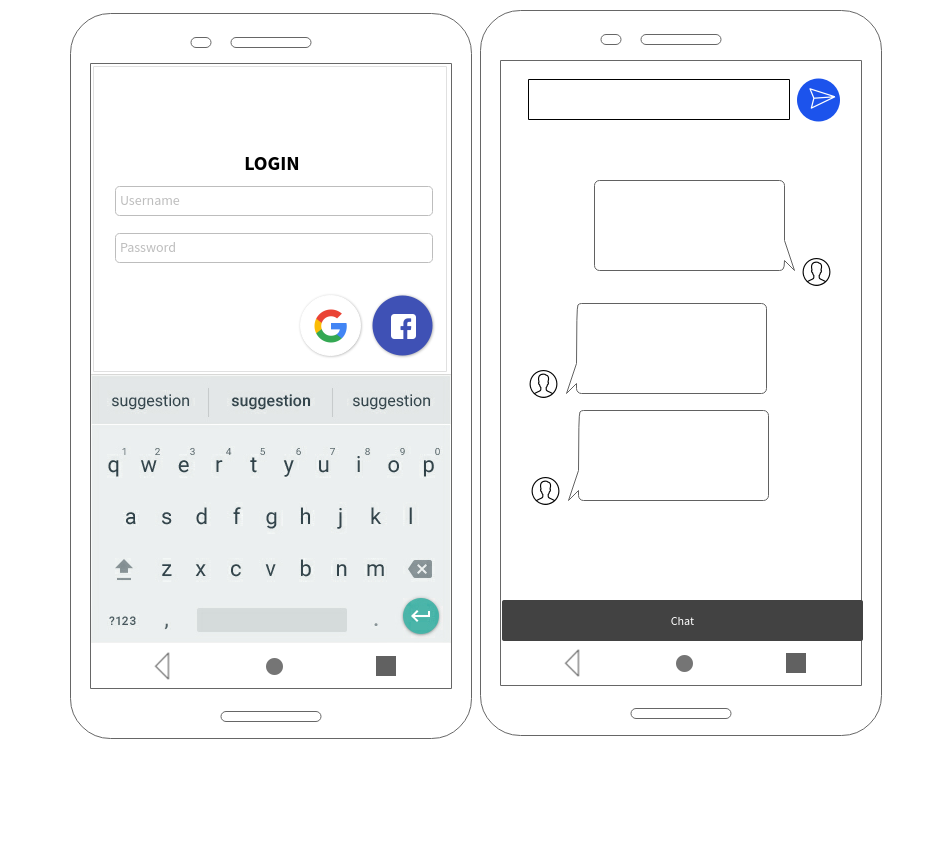
\includegraphics[height=7cm]{Figures/P1/example.jpeg}    
\end{center}
Las interacciones sociales de los Kwiis son bastante complejas, sus comunidades se construyen a partir de las amistades. Los Kwiis pueden construir sus propias listas de amigos en la Kwii Platform. Esta lista de amigos indica qué Kwiis considera un Kwii como su amigo. La amistad quiere decir, en la Kwii Platform, la capacidad de compartir información personal del Kwii (de su usuario asociado). Es así como se presentan dos tipos de perfiles, para todos los usuarios, uno que será compartido a nivel global, que indicará únicamente su identificador Kwii en la plataforma, y un usuario privado el cual podrá ser visto por los amigos del Kwii.
\begin{center}
    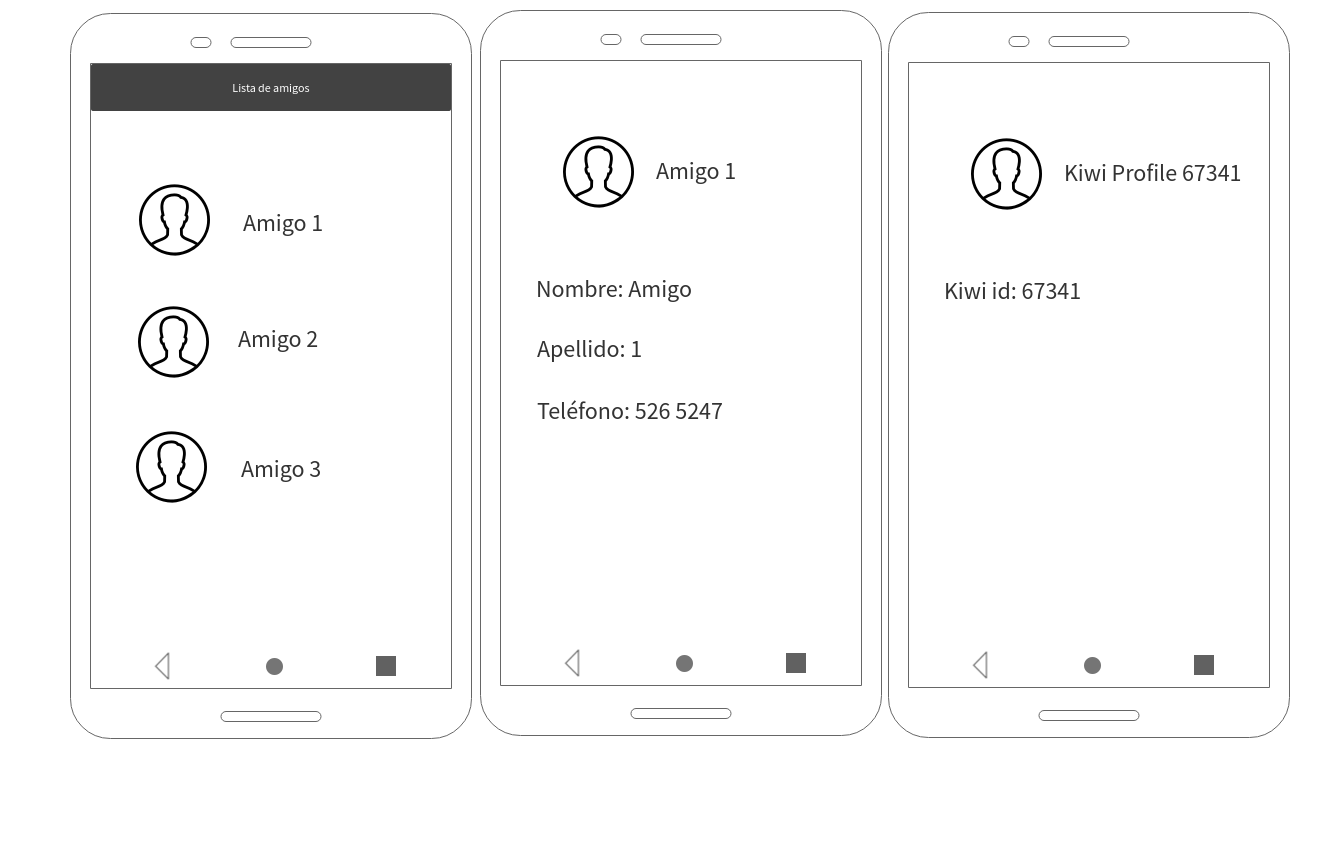
\includegraphics[height=7cm]{Figures/P1/example_2.jpeg}    
\end{center}
\subsubsection{Descripción de ideas para el sistema de software para trabajo futuro}
Los Kwiis son dotados de muy buena memoria, siendo capaces de recordar conversaciones que tuvieron con otros Kwiis hasta 5 años, sin embargo, también son muy buenos guardando secretos, ser grandes confidentes es la base de su compleja sociedad, así que si un amigo Kwii pide que olviden lo que le van a contar en una conversación en 5 minutos exactos, sus amigos Kwiis van a borrar toda evidencia de este evento pasados los 5 minutos exactos. En los chats individuales y grupales, los usuarios tienen la posibilidad de enviar mensajes con tiempo de expiración, y de eliminar, antes de pasados 10 minutos, los mensajes enviados sin expiración. Por defecto, todos los mensaje tienen una vigencia de 5 años.
\begin{center}
    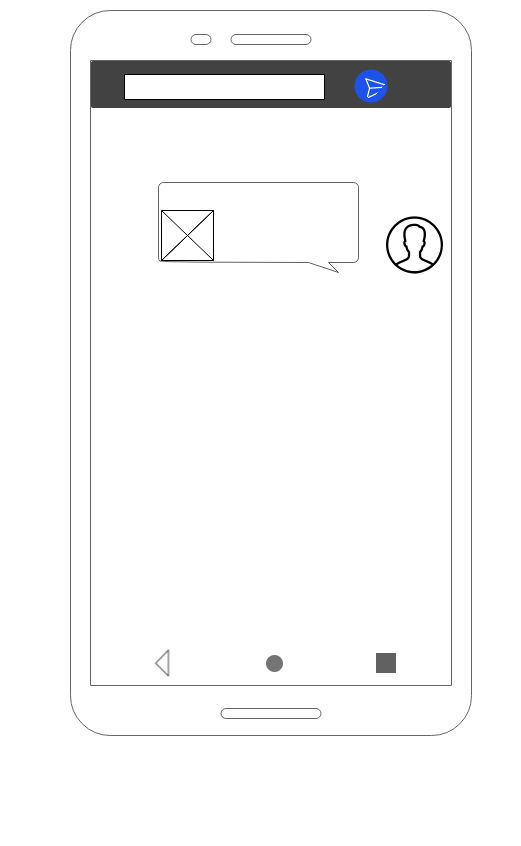
\includegraphics[height=7cm]{Figures/P1/example_3.jpeg}    
\end{center}
Los Kwiis son seres muy sociales, les gusta reunirse y no solo hablar desde la distancia, es por ello que los Kwiiers permiten a los Kwiis acercarse y encontrarse en cualquier lugar del mapa. Los usuarios pueden compartir en tiempo real su ubicación. Además, habilitada la opción de "encontrarse", los usuarios pueden recibir notificaciones sobre otros Kwiis cerca.
\begin{center}
    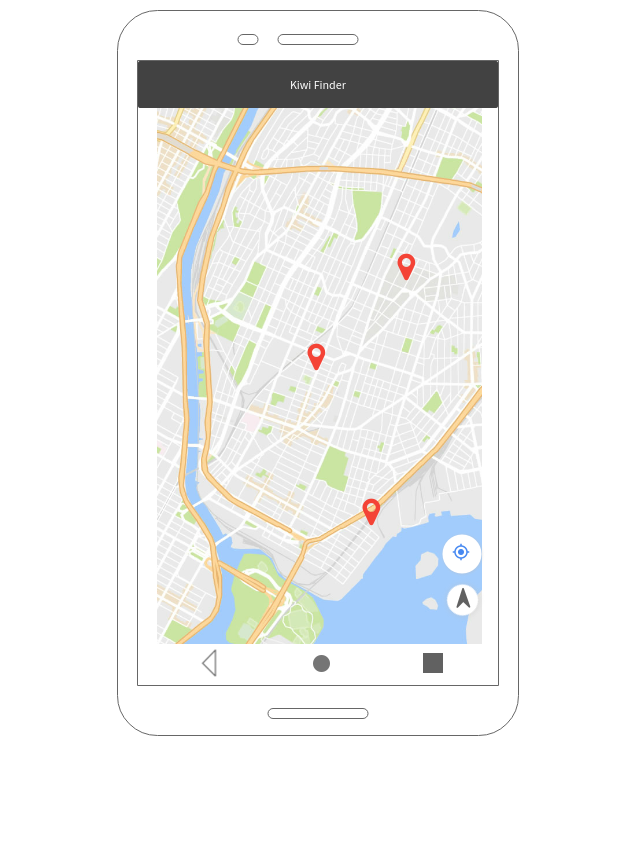
\includegraphics[height=7cm]{Figures/P1/example_4.jpeg}    
\end{center}
Además, los Kwiis tienen sistemas económicos complejos, es por esto que los Kwiiers permiten a los Kwiis hacer transacciones en KwiiCoins, la moneda principal de los Kwiis. Los usuarios, a través de la aplicación, podrán hacer transacciones en la moneda virtual KwiiCoin que será manejada por la plataforma. Un KwiiCoin equivale a un Peso Colombiano. Dos mil (2.000) KwiiCoins equivalen a una piragua en el Comedor Central de la Universidad Nacional de Colombia.
\begin{center}
    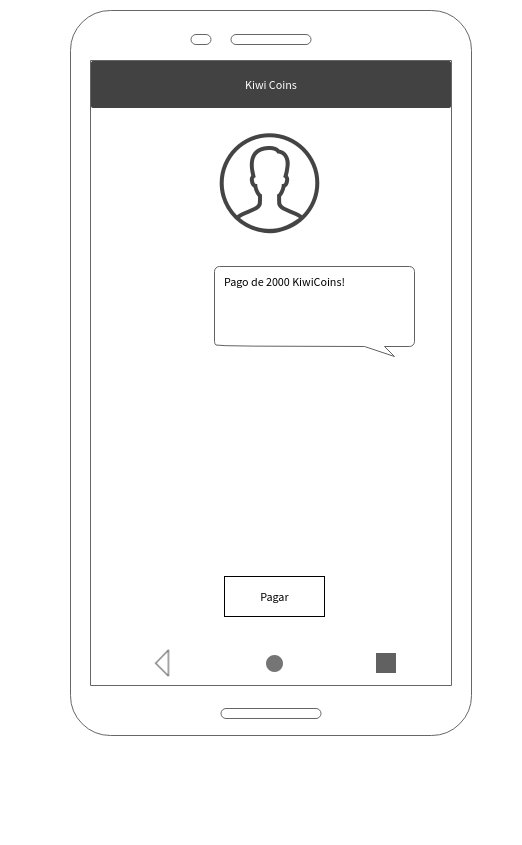
\includegraphics[height=7cm]{Figures/P1/example_5.jpeg}    
\end{center}
La compleja sociedad de los Kwiis ha construido en la Kwii Platform a los KwiiBots, Bots creados por otros Kwiis que les facilitan la vida. Ellos son capaces de hacer muy buenas conversaciones, se comportan como cualquier otro Kwii, pero un Kwii puede ser dueño de un único KwiiBot. Los usuarios dentro de la Kwii Platform pueden crear y adminitrar un único bot dentro de la aplicación. Dichos bots se comportarán como otros usuarios teniendo perfiles, pero sus perfiles son únicamente públicos.\\\\
En las sombras de la sociedad de los Kwiis se esconden los KwiiAdmins, que son entidades grandiosas que velan por la seguridad, expansión y continua mejora de la Kwii Platform. Aunque para los demás Kwiis ellos parecen Kwiis normales y corrientes, éstos Kwiis tienen acceso al sistema Kwii Platform en su totalidad. En el mundo de los humanos, los KwiiAdmins se les llaman desarrolladores.

\subsection{Ingeniería de requisitos}

En el estudio de ingeniería de requisitos, se encuentran las diversas historias de usuario, y dichas historias son desglosadas, exponiendo sus respectivos casos en el diagrama de casos de uso, además son consolidadas en una tabla de casos de uso y también son presentadas al detalle en las tablas de descripción de casos de uso.
\\\\
Finalmente es mostrado un conjunto de requisitos no funcionales, que garantizarán la calidad de la Kwii Platform.

\subsubsection{Identificación de los concerns y sus respectivos stakeholders}
Para exponer los stakeholders y sus respectivos concerns, se exponene las siguientes historias de usuario:

\begin{itemize}
    \item Usuarios de la aplicación (Kwiis)
    \begin{itemize}
        \item Como Kwii, yo debo poder registrarme en la aplicación, con el objetivo de poder volver a utilizar la aplicación desde otro dispositivo.
        \item Por supuesto, como Kwii, también debo poder iniciar sesión en la aplicación. Así podré recuperar mis datos cuando, por ejemplo, pierda mi celular.
        \item Es importante que con la aplicación pueda entrar en contacto con otras personas (Kwiis), es por eso que debería poder enviar mensajes en la aplicación.
        \item Para mí como usuario de la aplicación, es menester enviar mensajes no solo a otro usuario, sino a varios, para así fácilmente compartir mis ideas a varios otros usuarios a la vez.
        \item Es importante que la aplicación me notifique cuando otro usuario me escriba, para así, si tengo la posibilidad, poderle contestar de manera rápída.
        \item Como Kwii, usuario de la aplicación, debo poder hacer uso de los servicios de la aplicación desde mi computador o mi celular (inclusive desde ambos a la vez).
        \item A veces, como usuario, puedo ser bastante descuidado con los mensajes que envío, es por eso que me encantaría poder borrar mensajes enviados por error o descuido.
        \item Me gustaría que los demás usuarios puedan ver mi foto de perfil, para así poder ser identificado más fácil entre los otros usuarios.
        \item Algo de infromación personal como perfiles, también estaría bien, para poder personalizar mi cuenta.
        \item A veces, me es difícil encontrar personas cercanas con las que pueda compartir sin moverme demasiado de mi lugar de trabajo, mi casa, o donde simplemente esté en un momento dado, es por eso que me gustaría poder encontrar usuarios cercanos que estén usando la aplicación en el momento en el que yo la esté usando.
        \item También me gustaría poder pagar mis deudas utilizando una aplicación de pagos, para así no tener que usar dinero en efectivo o sencillamente no tener que retirar en un banco.
        \item Sería encantador poder hablar con algún tipo de bot o máquina dentro de la misma aplicación.
    \end{itemize}
    \item Equipo de desarrollo (KwiiAdmins)
    \begin{itemize}
        \item Para nosotros como equipo de desarrollo podría ser interesante extraer estadísticas de la aplicación, con el fin de observar el comportamiento de los usuarios y analizar dónde puede mejorar la aplicación.
    \end{itemize}
\end{itemize}

\subsubsection{Especificación de los requisitos funcionales}

Se presentan a continuación los diagramas de casos de uso que resumen las historias de casos de uso presentadas anteriormente. En el diagrama, los casos de uso que no hacen parte de la implementación de la primera entrega son señalados.
\begin{center}
    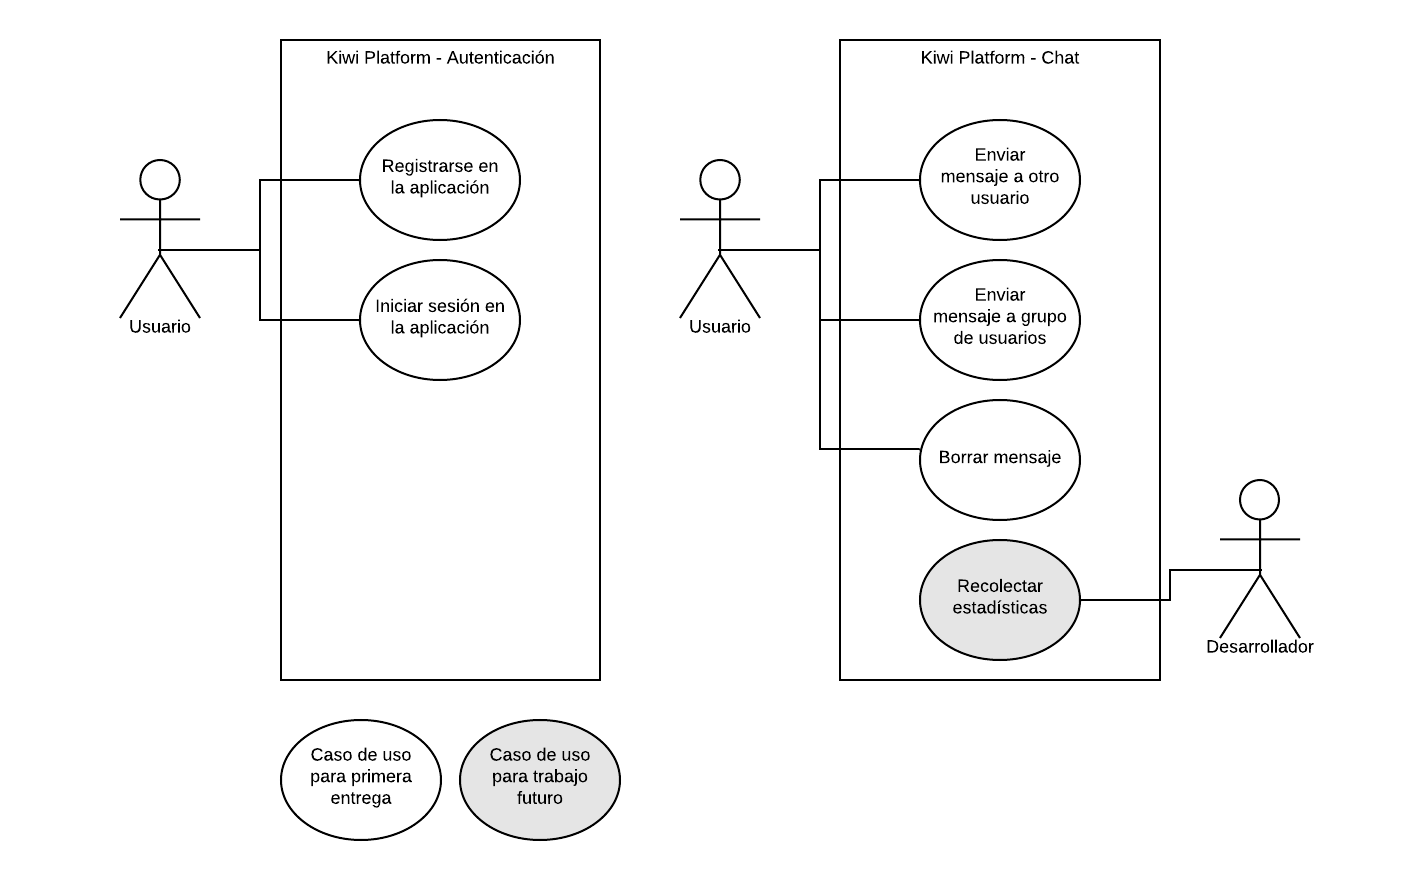
\includegraphics[width=15cm]{Figures/P1/cases_diagram_1.png}
\end{center}
\begin{center}
    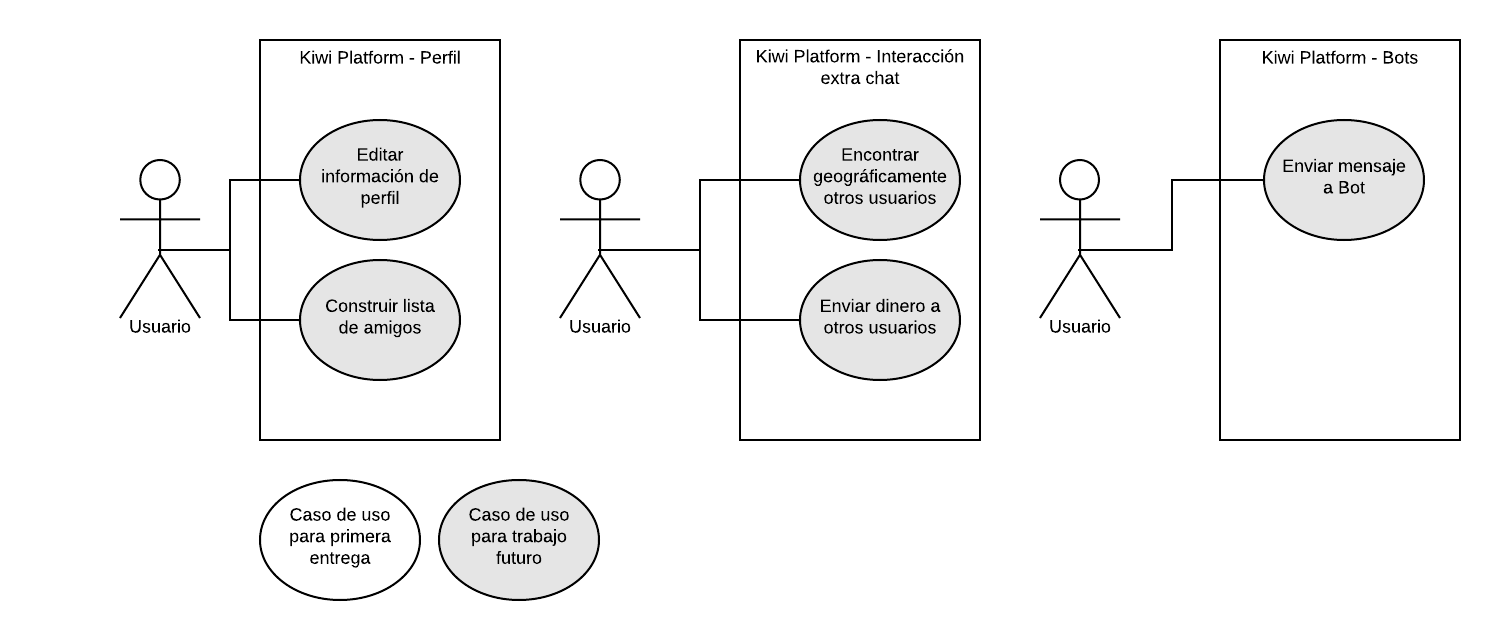
\includegraphics[width=15cm]{Figures/P1/cases_diagram_2.png}
\end{center}
Ahora, mostramos la tabla de casos de uso, para ellos, a cada uno le asignamos un identificador, su nombre y actor, además de lo que es considerado la "complejidad" de implementar para el equipo de desarrollo, la "prioridad" de implementar la funcionalidad y finalmente, si esta para esta funcionalidad, es implementada su lógica en la primer entrega, o si es considerada trabajo futuro.

\begin{center}
\begin{tabular}{|c|c|c|c|c|c|}
\hline
ID & Nombre & Actor & Complejidad & Prioridad & Primera entrega \\
\hline
1 & \makecell{Registrarse en la\\ aplicación} & Usuario & Media & Alta & Sí \\
\hline
2 & \makecell{Iniciar\\ sesión} & Usuario & Media & Alta & Sí \\
\hline
3 & \makecell{Enviar mensaje\\ a otro usuario} & Usuario & Alta & Alta & Sí \\
\hline
4 & \makecell{Enviar mensaje\\ a grupo de usuarios} & Usuario & Muy alta & Alta & Sí \\
\hline
5 & \makecell{Recibir notificaciones\\ de la aplicación} & Usuario & Alta & Alta & Sí \\
\hline
6 & \makecell{Borrar \\mensajes} & Usuario & Alta & Media & No \\
\hline
7 & \makecell{Editar información\\ de mi perfil} & Usuario & Media & Media & No \\
\hline
8 & \makecell{Construir lista\\ de amigos} & Usuario & Media & Baja & No \\
\hline
9 & \makecell{Encontrar usuarios\\ geográficamente} & Usuario & Muy alta & Muy
baja & No \\
\hline
10 & \makecell{Enviar dinero\\ a otros usuarios} & Usuario & Muy alta & Muy baja & No \\
\hline
11 & \makecell{Enviar mensajes\\ a bot} & Usuario & Muy alta & Baja & No \\
\hline
12 &  \makecell{Recolectar estadísitcas\\ sobre el uso de la aplicación} & Desarrollador & Media & Media & No\\
\hline
\end{tabular}
\end{center}

Ahora, presentaremos los casos de uso de forma más amplia, escribiendo la descripción de estos.

\begin{center}
\begin{tabular}{|p{0.1\textwidth}|p{0.8\textwidth}|}
\hline
\textbf{ID} & 1\\ 
\hline
Nombre & Registrarse en la aplicación\\
\hline
Descripción & Un usuario puede entrar a la aplicación y crear un perfil, lo que significa poder registrarse dentro de la plataforma para así poder llevar registro de las conversaciones que ha tenido y demás información importante dentro de su perfil \\
\hline
\end{tabular}
\vspace{2mm}

\begin{tabular}{|p{0.1\textwidth}|p{0.8\textwidth}|}
\hline
\textbf{ID} & 2 \\ 
\hline
Nombre & Iniciar sesión dentro de la aplicación \\
\hline
Descripción & Un usuario puede entrar a la aplicación con su usuario y contraseña si son correctos\\ 
\hline
\end{tabular}
\vspace{2mm}

\begin{tabular}{|p{0.1\textwidth}|p{0.8\textwidth}|}
\hline
\textbf{ID} & 3\\
\hline
Nombre & Enviar mensaje a otro usuario\\ 
\hline
Descripción & Un usuario puede enviarle un mensaje de manera privada a otro usuario que esté registrado en la aplicación \\
\hline
\end{tabular}
\vspace{2mm}

\begin{tabular}{|p{0.1\textwidth}|p{0.8\textwidth}|}
\hline
\textbf{ID} & 4\\ 
\hline
Nombre & Enviar mensaje a grupo de usuarios\\ 
\hline
Descripción & Un usuario puede enviarle un mensaje de manera privada a un grupo de usuarios registrado en la aplicación\\
\hline
\end{tabular}
\vspace{2mm}

\begin{tabular}{|p{0.1\textwidth}|p{0.8\textwidth}|}
\hline
\textbf{ID} & 5\\
\hline
Nombre & Recibir notificaciones de la aplicación\\
\hline
Descripción & Un usuario puede recibir notificaciones en el cliente donde esté usando la aplicación \\ 
\hline
\end{tabular}
\vspace{2mm}

\begin{tabular}{|p{0.1\textwidth}|p{0.8\textwidth}|}
\hline
\textbf{ID} & 6\\
\hline
Nombre & Borrar mensajes\\
\hline
Descripción & Un usuario puede borrar mensajes enviados por él y que ya no queden registrados en los historiales\\
\hline
\end{tabular}
\vspace{2mm}

\begin{tabular}{|p{0.1\textwidth}|p{0.8\textwidth}|}
\hline
\textbf{ID} & 7\\
\hline
Nombre & Editar información de mi perfil\\
\hline
Descripción & Un usuario puede editar y actualizar la información relacionada a su cuenta \\ 
\hline
\end{tabular}
\vspace{2mm}

\begin{tabular}{|p{0.1\textwidth}|p{0.8\textwidth}|}
\hline
\textbf{ID} & 8\\
\hline
Nombre & Construir lista de amigos\\
\hline
Descripción & Un usuario puede manejar una lista de amigos (usuarios registrados en la aplicación) \\ 
\hline
\end{tabular}
\vspace{2mm}

\begin{tabular}{|p{0.1\textwidth}|p{0.8\textwidth}|}
\hline
\textbf{ID} & 9\\
\hline
Nombre & Encontrar usuarios geográficament\\
\hline
Descripción & Un usuario puede encontrar a otros usuarios por medio de la geolocalización\\ 
\hline
\end{tabular}
\vspace{2mm}

\begin{tabular}{|p{0.1\textwidth}|p{0.8\textwidth}|}
\hline
\textbf{ID} & 10\\
\hline
Nombre & Enviar dinero a otros usuarios\\
\hline
Descripción & Un usuario puede enviar dinero a otros usuarios por medio de una cartera electrónica \\
\hline
\end{tabular}
\vspace{2mm}

\begin{tabular}{|p{0.1\textwidth}|p{0.8\textwidth}|}
\hline
\textbf{ID} & 11\\
\hline
Nombre & Enviar mensajes a un bot\\
\hline
Descripción & Un usuario puede tener conversaciones con bots creados por otros usuarios \\
\hline
\end{tabular}
\vspace{2mm}

\begin{tabular}{|p{0.1\textwidth}|p{0.8\textwidth}|}
\hline
\textbf{ID} & 12\\
\hline
Nombre & Recolectar estadísticas sobre el uso de la aplicación\\
\hline
Descripción & Los desarrolladores podrán tener la capacidad de recolectar información del uso de la aplicación y generar estadísticas\\
\hline
\end{tabular}
\end{center}

\subsubsection{Especificación de los requisitos no funcionales}
Para garantizar la calidad de la Kwii Platform, son listadas los siguientes requisitos no funcionales junto por qué es considerado un requisito para el sistema.
\begin{itemize}
    \item El sistema debe está implementado haciendo uso de una arquitectura de microservicios para facilitar su escalabilidad e interoperabilidad.
    \item La funcionalidad de la plataforma se distribuye en 5 microservicios los cuales funcionan cada uno con una tecnologia diferente, estos son:
    \begin{itemize}
        \item Componente Usuarios \\
        Lenguaje usado: Ruby \\
        Framework usado: Ruby on Rails \\
        Base de Datos: PosgreSQL
        
        \item Componente Autenticación \\
        Lenguaje usado: Javascript \\
        Framework usado: Express \\
        Base de Datos: Redis
        
        \item Componente Chat \\
        Lenguaje usado: Python \\
        Framework usado: Django \\
        Base de Datos: MongoDB
        
        \item Componente ChatRoom \\
        Lenguaje usado: Java \\
        Framework usado: Maven \\
        Base de Datos: MySQL
        
        \item Componente Notificaciones \\
        Lenguaje usado: Go \\
        Framework usado: Rush \\
        Base de Datos: Redis
    \end{itemize}
\end{itemize}